\chapter{Scenario(s)}

We will propose a simple application to begin with and see how the scheduler behaves, then we will show several
schedules for random sets of tasks.

The scenario is about a factory in which there are a lot of shortcircuits happening. Each shortcircuit has a 10\% chance of
igniting a fire, and each shortcircuit has 10\% chance of occuring in any large enough interval of time. We would like to have
a level-based alarm system, where the network detects a shortcircuit and only then checks for immediate increases in temperature.
This application can be obviously extended in multiple ways (more wireless nodes, more types of sensors). The factory uses
220V dual-phase AC.

The system proposed has one Sparrow Power node and two AVR Raven\texttrademark$\:$ boards, and is broken down into 6 tasks.

\begin{figure}
  \centering
  \subfloat[The Task DAG]{\label{fig:fire1}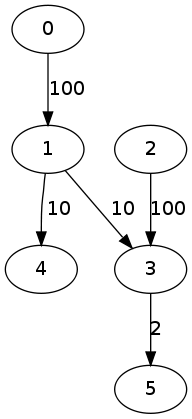
\includegraphics[width=0.2\textwidth]{scenario/fire1.png}}                
  \subfloat[The Allocated Tasks]{\label{fig:fire2}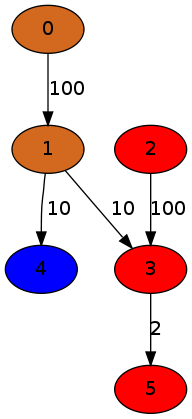
\includegraphics[width=0.2\textwidth]{scenario/fire2.png}}
  \caption{The scenario}
\end{figure}

The result is that the voltage related tasks are assigned to the Sparrow Power, while the other tasks are split in two:
Shortcircuit alarm is delegated to one Raven, while the other checks for increases in temperature and has a fire alert.



\begin{table}[ht]
 \centering
\begin{tabular}{|l|c|c|c|}
\hline
Task name & Task no. & Frequency & Affinity\\
\hline
Voltage sampling & 0 & 1 & Sparrow Power\\
\hline
Voltage decrease detection & 1 & 1 & Sparrow Power\\
\hline
Temperature sensing & 2 & 1 & AVR Raven \\
\hline
Fire detection & 3 & 1 & AVR Raven \\
\hline
Shortcircuit alarm & 4 & 1 & AVR Raven  \\
\hline
Fire alarmn & 5 & 1 & AVR Raven \\
\hline
\end{tabular}
\caption{Tasks of scenario}
\label{tab:scenario}
\end{table}

\begin{figure}
  \centering
  \label{fig:rand1}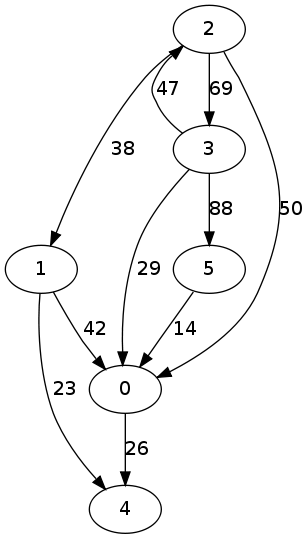
\includegraphics[width=0.4\textwidth]{scenario/rand1.png}
  \label{fig:rand2}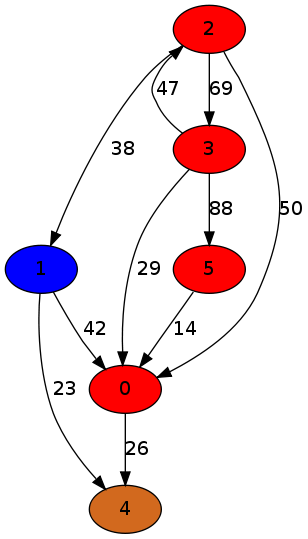
\includegraphics[width=0.4\textwidth]{scenario/rand2.png}
  \caption{A random scenario}
\end{figure}